%%%%%%%%%%%%%%%%%%%%%%%%%%%%%%%%%%%%%%%%%%%%%%%%%%%%%%%%%%%%%%%%%%%%%%%%%%%
%
% Plantilla para un artículo en LaTeX en español.
%
%%%%%%%%%%%%%%%%%%%%%%%%%%%%%%%%%%%%%%%%%%%%%%%%%%%%%%%%%%%%%%%%%%%%%%%%%%%

% Qué tipo de documento estamos por comenzar:
\documentclass[a4paper]{article}
% Esto es para que el LaTeX sepa que el texto está en español:
\usepackage[spanish]{babel}
\selectlanguage{spanish}
% Esto es para poder escribir acentos directamente:
\usepackage[utf8]{inputenc}
\usepackage[T1]{fontenc}



%% Asigna un tamaño a la hoja y los márgenes
\usepackage[a4paper,top=3cm,bottom=2cm,left=3cm,right=3cm,marginparwidth=1.75cm]{geometry}

%% Paquetes de la AMS
\usepackage{amsmath, amsthm, amsfonts}
%% Para añadir archivos con extensión pdf, jpg, png or tif
\usepackage{graphicx}
\usepackage[colorinlistoftodos]{todonotes}
\usepackage[colorlinks=true, allcolors=blue]
%% Para añadir partituras
%%\usepackage{musixtex}
%%\usepackage{biblatex}
{hyperref}

%% Primero escribimos el título
\title{La guitarra panzona \\
    \large Un estudio desde el diseño sonoro}
\author{Allan Ulises Zepeda Ibarra\\
\small Taller de Lauderia Ibarra\\
\small 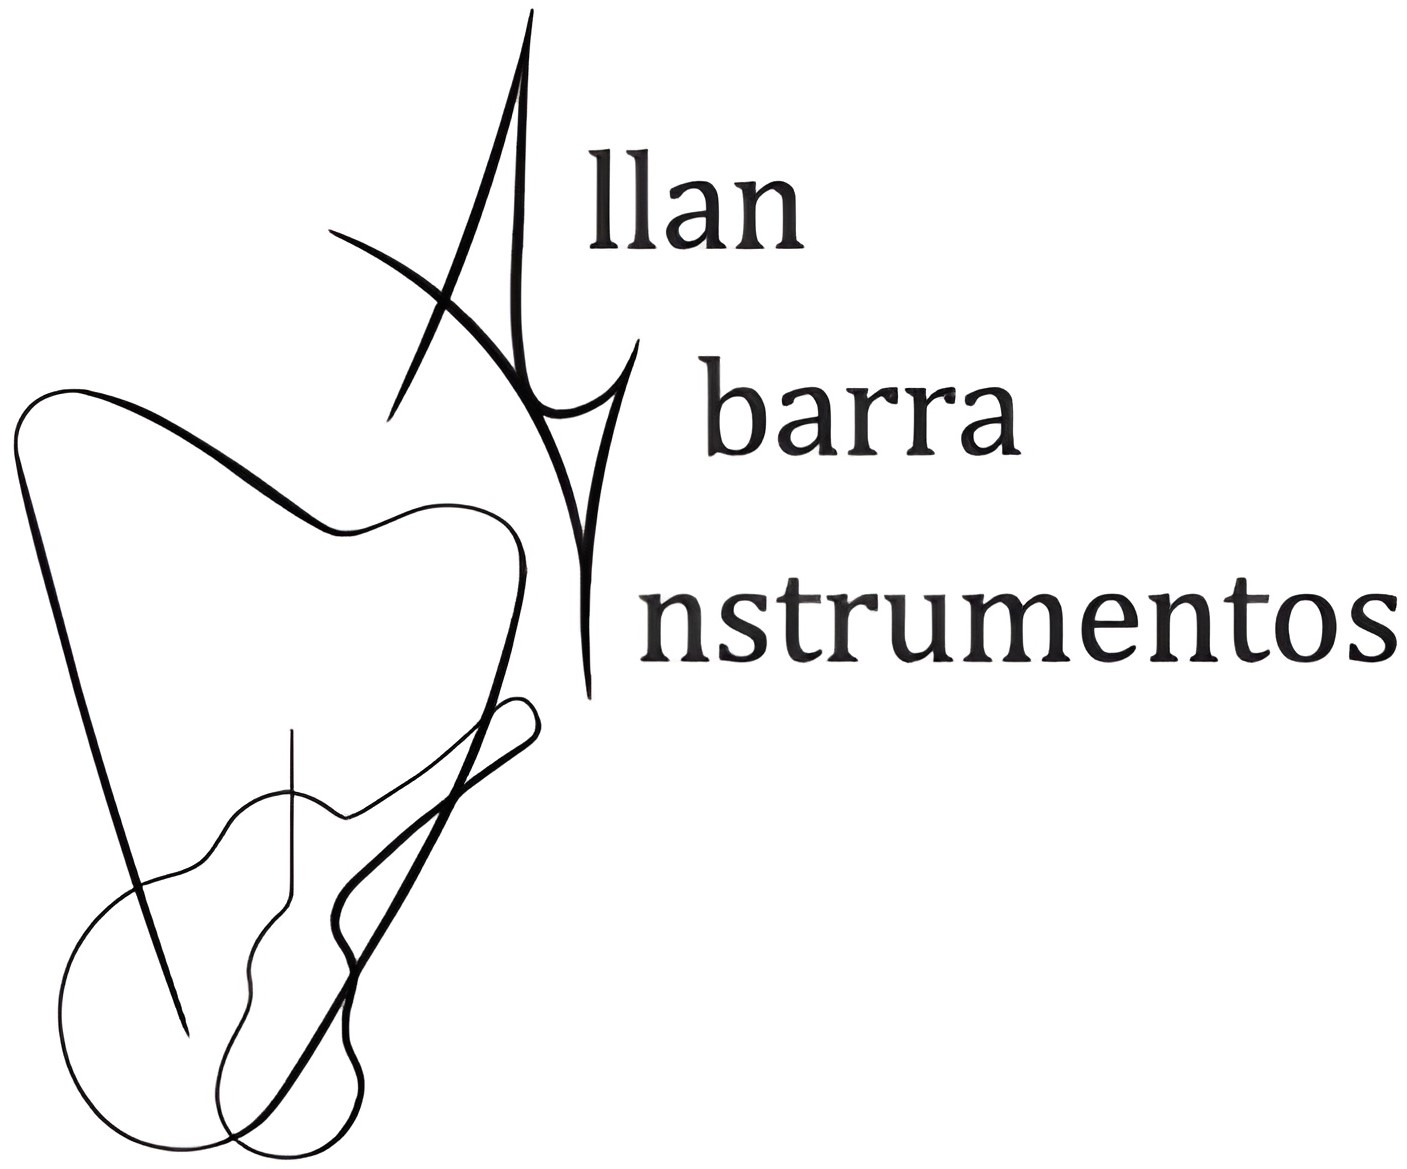
\includegraphics[width=0.25\textwidth]{./img/logo.jpg}\\
  \small allanibarramusica@gmail.com\\
  \small Ciudad de México
  \date{}
}

%% Después del "preámbulo", podemos empezar el documento

\begin{document}
%% Hay que decirle que incluya el título en el documento
\maketitle

%% Aquí podemos añadir un resumen del trabajo (o del artículo en su caso) 
\begin{abstract}

\end{abstract}

%% Iniciamos "secciones" que servirán como subtítulos
%% Nota que hay otra manera de añadir acentos
\section{Breve historia de la guitarra Túa, panzona o tamborina}
\cite{martinez-ayala-2022}

\section{Conceptos usados para el analisis y diseño de la guitarra panzona}

\subsection{El Tanto}




\subsection{La escala y la perspectiva isometrica}
% * <stephmigoni@gmail.com> 2018-02-08T19:23:33.559Z:
% 
% Esto es un comentario de prueba
% 
% 


\section{Organologia de la guitarra panzona y caracteristicas}
\subsection{Tapa armonica}
\subsubsection{puente}
\subsubsection{boca}
\subsection{caja armonica}
\subsubsection{fondo}
\subsection{cuerdas}
\subsection{brazo}
\subsubsection{diapason}
\subsubsection{pala}
\section{analisis de la guitarra panzona}
\subsection{Guitarra 1 Ranferi}
\subsection{Guitarra 2 Tavira}
\subsection{Guitarra 3 Juan Reynoso}
\subsection{Guitarra 4 Agustin villa}
\subsection{Guitarra 5 Conjunto Ajuchitlan}
\section{La construccion de la Guitarra panzona ``La Chimali''}


\subsection{El diseño}



\subsection{La construccion}


\subsection{El resultado}


\subsection{Conclusiones}
\bibliographystyle{acm}
\bibliography{LaGuitarraPanzona}

\end{document}